\documentclass[10pt]{article}
\usepackage{icmlko}

\icmlmeta{IP 파운데이션 월드모델}{316}{이 판은 도메인 순서를 읽은 적이 없다}{노트 315의 검사를 짝 비교 일곱에 소급해 걸었다 --- 하나도 문턱 근처에 못 간다}

\begin{document}

\twocolumn[
\icmlheader

\begin{abstract}
노트 315가 \texttt{lab/ordering.py} 를 만들고 ``옛 노트의 순서 주장''을 남겼다.
이 판이 지금 들고 있는 짝 비교에 소급해 걸었다. \textbf{일곱 중 하나도
문턱(선 쌍 80\%) 근처에 못 간다.} 문턱 40 대 15(노트 296) 17/45(38\%) ·
\texttt{fund\_cat}(노트 309) 15/45(33\%) · \texttt{fund\_cat}$\cdot$F6
4/45(9\%) · \texttt{mkt} 축(노트 285) \textbf{0/45} · 팝업 전용 축
\textbf{0/45} · LOO$\cdot$F18(노트 310) 5/28(18\%) · LOO$\cdot$F6(노트 314)
1/28(4\%). \textbf{이웃 쌍은 일곱 중 다섯에서 0 이다.} 그러니 노트 310이
특별히 운이 나빴던 게 아니라 \textbf{이 판에서 도메인 순서는 원래 안 읽힌다.}
까닭은 단순하다 --- 도메인별 짝SE 가 웹툰 0.004 에서 아이돌 0.056 까지
\textbf{열네 배} 벌어져 있고, 도메인 차 자체가 대부분 문턱 아래다.
\textbf{읽을 수 있는 것은 따로 있다}: 도메인 \emph{하나}의 값(짝SE 를 붙여),
계열로 묶은 값(노트 313의 ``검색 셋 대 달력 여섯''), 무리로 묶은 값(노트 311의
``나무 대 선형''). 오늘 문턱을 넘은 결론은 전부 그 셋 중 하나였다.
\textbf{순서만 아니었다.}
\end{abstract}
]

\section{소급해 걸었다}

노트 315가 짝짝이 확률로 순서의 안정성을 재는 도구를 만들었다. 이 판이
지금 들고 있는 짝 비교에 걸었다.

\begin{figure*}[t]
\centering
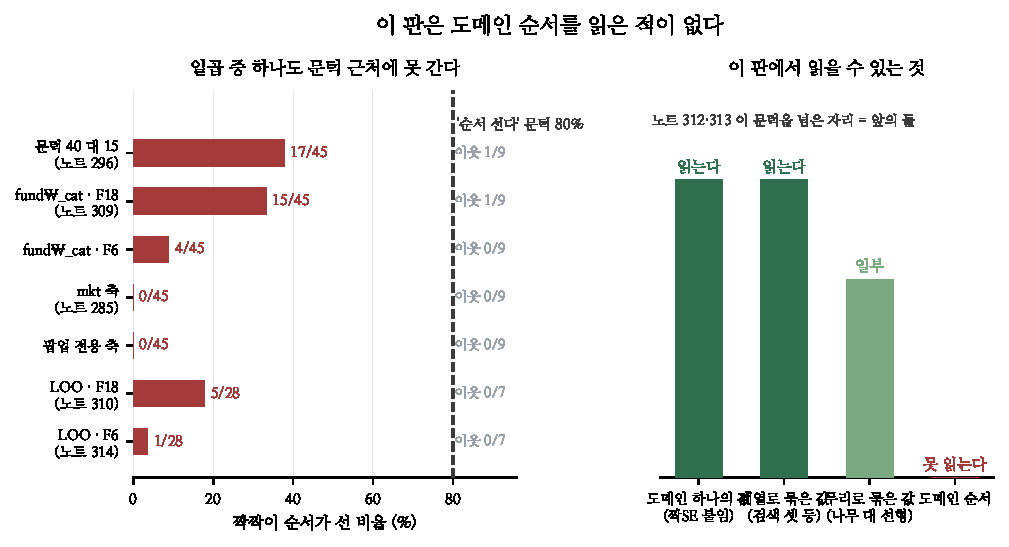
\includegraphics[width=\textwidth]{figs/never.pdf}
\caption{왼쪽 --- 짝 비교마다 순서가 선 쌍의 비율. 오른쪽 --- 이 판에서
읽을 수 있는 주장의 종류.}
\end{figure*}

\begin{center}\footnotesize
\begin{tabular}{lrrl}
\hline
비교 & 선 쌍 & 이웃 & 판정 \\
\hline
문턱 40 대 15 (노트 296) & 17/45 & 1/9 & 못 읽는다 \\
\texttt{fund\_cat} · F18 (노트 309) & 15/45 & 1/9 & 못 읽는다 \\
LOO · F18 (노트 310) & 5/28 & 0/7 & 못 읽는다 \\
\texttt{fund\_cat} · F6 & 4/45 & 0/9 & 못 읽는다 \\
LOO · F6 (노트 314) & 1/28 & 0/7 & 못 읽는다 \\
\texttt{mkt} 축 (노트 285) & \textbf{0/45} & 0/9 & 못 읽는다 \\
팝업 전용 축 & \textbf{0/45} & 0/9 & 못 읽는다 \\
\hline
\end{tabular}
\end{center}

\textbf{제일 높은 것이 38\%다.} 그리고 \textbf{이웃 쌍은 일곱 중 다섯에서
0 이다} --- 순서를 읽을 때 실제로 쓰는 것이 이웃 쌍인데 그게 하나도 안 선다.

\section{왜 원래 안 읽히나}

\begin{center}\small
\begin{tabular}{lrr}
\hline
도메인 & 유보 & 짝SE(전형) \\
\hline
웹툰 & 711 & 0.004 \\
애니 & 606 & 0.006 \\
모바일 & 441 & 0.004 \\
세계애니 & 300 & 0.011 \\
도서 & 163 & 0.030 \\
아이돌 & 25 & \textbf{0.056} \\
\hline
\end{tabular}
\end{center}

\textbf{짝SE 가 열네 배 벌어져 있다.} 아이돌의 차 하나가 웹툰의 차 열넷과
같은 불확실성을 갖는다. 그런 값들을 크기 순으로 늘어놓으면 \textbf{작은
도메인이 위아래 어디든 갈 수 있다.} 노트 310에서 아이돌이 꼴찌였고 노트 314
에서는 다섯째였다.

\paragraph{그리고 도메인 차 자체가 대부분 문턱 아래다} 일곱 비교에서
$|t|{>}$문턱인 도메인이 \textbf{전부 0개}였다. 못 가르는 값이 아홉 개면
그 아홉의 순서도 못 가른다 --- 노트 314의 규약 그대로다.

\section{읽을 수 있는 것}

오늘 문턱을 넘은 결론을 모아 보면 종류가 셋이다.

\begin{center}\scriptsize
\begin{tabular}{ll}
\hline
종류 & 예 (노트) \\
\hline
도메인 \emph{하나}의 값 & 도서 빌림 $+$0.1143, $t{=}{-}3.79$ (312) \\
계열로 묶은 값 & 검색 $+$0.1132, 달력 $-$0.0051 (313) \\
무리로 묶은 값 & 나무 짝SE 0.042$\sim$0.048, 선형 0.030$\sim$0.034 (311) \\
\hline
\textbf{도메인 순서} & \textbf{없음} \\
\hline
\end{tabular}
\end{center}

\textbf{순서만 아니었다.} 셋 다 \emph{묶어서} 한 값을 만들거나 \emph{하나}만
집는다. 여럿을 동시에 줄 세우는 주장은 이 판의 분해능 밖이다.

\paragraph{그래서 규약을 하나 더} 도메인별 표를 낼 때 \textbf{크기 순으로
정렬하지 않는다.} 정렬 자체가 순서 주장으로 읽힌다 --- 노트 310이 정확히
그렇게 시작했다. 이름 순이나 유보 행 순으로 낸다.

\paragraph{남은 것}
\begin{center}\small
\begin{tabular}{ll}
\hline
갈래 & 왜 \\
\hline
정확 셈으로 & 재추출을 저장하면 상관이 산다 \\
``상위 $k$'' 문턱 & 순서보다 약한 주장은 몇 쌍이면 되나 \\
풀링 총 이득 & 돌고 있다 --- 오늘의 제일 큰 물음 \\
표를 이름 순으로 & 정렬이 주장이 되지 않게 \\
\hline
\end{tabular}
\end{center}

\paragraph{규약} \textbf{도구를 만들면 옛것에 소급해 걸어라.} 노트 315가
도구를 만들 때는 노트 310 하나를 잡았는데, 걸어 보니 \textbf{일곱 전부}가
같은 상태였다. \textbf{한 번 틀린 것이 아니라 늘 그랬다} --- 다만 지금까지는
순서 위에 결론을 세운 적이 (노트 310 말고는) 없어서 드러나지 않았다.
\textbf{안 쓴 것과 못 쓰는 것은 다르고, 이제 못 쓴다는 것을 안다.}

\end{document}
